\documentclass[11pt,class=report,crop=false]{standalone}
\usepackage[screen]{../python}
\begin{document}

% Commande spécifique
\newcommand{\badletter}[1]{\underline{\textcolor{red}{#1}}}



%====================================================================
\chapitre{Images dynamiques}
%====================================================================

\objectifs{Nous allons déformer des images. En répétant ces déformations, les images deviennent brouillées. Mais par miracle au bout d'un certain nombre de répétitions l'image de départ réapparaît !}

\index{image}


\insertvideo{WXGci8trILg}{Images dynamiques - partie 1}

\insertvideo{DlZyWbXkotM}{Images dynamiques - partie 2}


%%%%%%%%%%%%%%%%%%%%%%%%%%%%%%%%%%%%%%%%%%%%%%%%%%%%%%%%%%%%%%%%
%%%%%%%%%%%%%%%%%%%%%%%%%%%%%%%%%%%%%%%%%%%%%%%%%%%%%%%%%%%%%%%%

\begin{cours}[Transformation du photomaton]

On part d'un tableau $n\times n$, avec $n$ pair, chaque élément du tableau représente un pixel. Les lignes sont indexées de $i=0$ à $i=n-1$, les colonnes de $j=0$ à $j=n-1$.
À partir de cette image on calcule une nouvelle image en déplaçant chaque pixel selon une transformation, appelée \defi{transformation du photomaton}.

On découpe l'image de départ selon des petits carrés de taille $2\times2$.
Chaque petit carré est donc composé de quatre pixels. On envoie chacun de ces pixels à quatre endroits différents de la nouvelle image :
le pixel en haut à gauche reste dans une zone en haut à gauche, le pixel en haut à droite du petit carré, s'envoie dans une zone en haut à droite de la nouvelle image,...

\myfigure{0.7}{
\tikzinput{fig-images-1}
}

Par exemple le pixel en position $(1,1)$ (symbolisé par la lettre \mot{D}) est envoyé en position $(4,4)$.

\medskip

Explicitons ce principe par des formules. Pour chaque couple $(i,j)$, on calcule son image $(i',j')$ par la transformation du photomaton selon les formules suivantes :
\begin{itemize}
  \item Si $i$ et $j$ sont pairs : $(i',j') = (i//2,j//2)$.
  \item Si $i$ est pair et $j$ est impair : $(i',j') = (i//2,(n+j)//2)$.  
  \item Si $i$ est impair et $j$ est pair : $(i',j') = ((n+i)//2,j//2)$.
  \item Si $i$ et $j$ sont impairs : $(i',j') = ((n+i)//2,(n+j)//2)$.
\end{itemize}


\medskip

Voici un exemple d'un tableau $4\times 4$ avant (à gauche) et après (à droite) la transformation du photomaton. 
$$\begin{array}{cccc} 
  1& 2& 3& 4\\ 
  5& 6& 7& 8\\  
  9&10&11&12\\  
 13&14&15&16  
\end{array}\qquad\qquad  
\begin{array}{cccc} 
  1& 3& 2& 4\\  
  9&11&10&12\\  
  5& 7& 6& 8\\  
 13&15&14&16
\end{array}$$

Voici une image $256 \times 256$ et sa première transformation :

\begin{center}
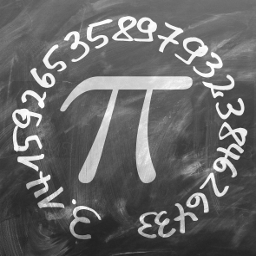
\includegraphics[scale=\myscale,scale=0.4]{images_fiche/pi_gimp_new_photo_0.png}\qquad\qquad
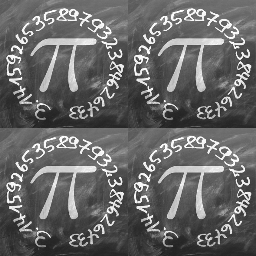
\includegraphics[scale=\myscale,scale=0.4]{images_fiche/pi_gimp_new_photo_1.png}
\end{center}

Voici ce qui se passe si on répète plusieurs fois la transformation du photomaton :
\begin{center}
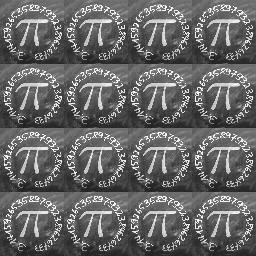
\includegraphics[scale=\myscale,scale=0.3]{images_fiche/pi_gimp_new_photo_2.png}\qquad
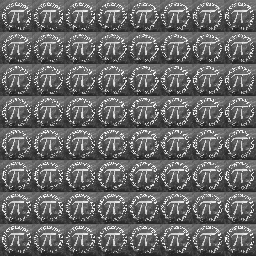
\includegraphics[scale=\myscale,scale=0.3]{images_fiche/pi_gimp_new_photo_3.png}\qquad
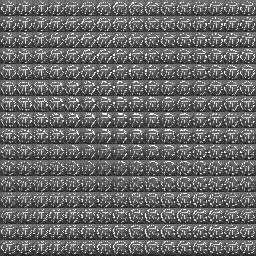
\includegraphics[scale=\myscale,scale=0.3]{images_fiche/pi_gimp_new_photo_4.png}
\end{center}
\begin{center}
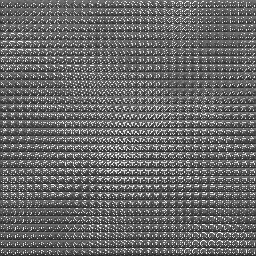
\includegraphics[scale=\myscale,scale=0.3]{images_fiche/pi_gimp_new_photo_5.png}\qquad
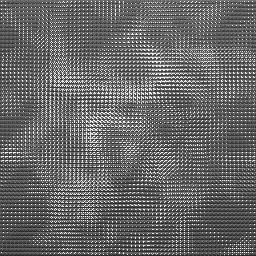
\includegraphics[scale=\myscale,scale=0.3]{images_fiche/pi_gimp_new_photo_6.png}\qquad
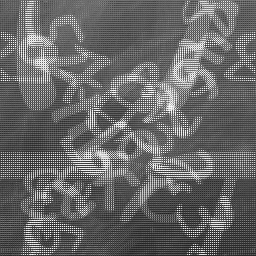
\includegraphics[scale=\myscale,scale=0.3]{images_fiche/pi_gimp_new_photo_7.png}\qquad
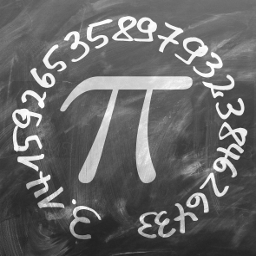
\includegraphics[scale=\myscale,scale=0.3]{images_fiche/pi_gimp_new_photo_8.png}
\end{center}
L'image devient de plus en plus brouillée, mais au bout d'un certain nombre de répétitions de la transformation, on retombe sur l'image de départ !
\end{cours}




%%%%%%%%%%%%%%%%%%%%%%%%%%%%%%%%%%%%%%%%%%%%%%%%%%%%%%%%%%%%%%%%
% Activité 1 - Transformation du photomaton
%%%%%%%%%%%%%%%%%%%%%%%%%%%%%%%%%%%%%%%%%%%%%%%%%%%%%%%%%%%%%%%%


\begin{activite}[Transformation du photomaton]

\objectifs{Objectifs : programmer la transformation du photomaton qui décompose une image en sous-images. Lorsque l'on itère cette transformation l'image se déstructure petit à petit, puis d'un coup se reforme !}



\begin{enumerate}
  \item Programme une fonction \ci{transformation(i,j,n)} qui met en 
  \oe uvre la formule de la transformation du photomaton et renvoie les coordonnées $(i',j')$ de l'image du pixel $(i,j)$.
  
  Par exemple \ci{transformation(1,1,8)} renvoie \ci{(4,4)}.
  
  \item Programme une fonction \ci{photomaton(tableau)} qui renvoie le tableau calculé après transformation.

Par exemple le tableau de gauche est transformé en le tableau de droite.
$$\begin{array}{cccc} 
  1& 2& 3& 4\\ 
  5& 6& 7& 8\\  
  9&10&11&12\\  
 13&14&15&16  
\end{array}\qquad\qquad
\begin{array}{cccc} 
  1& 3& 2& 4\\  
  9&11&10&12\\  
  5& 7& 6& 8\\  
 13&15&14&16
\end{array}$$

  \emph{Indications.} Tu peux initialiser un nouveau tableau par la commande :  
  \mycenterline{\ci{nouv_tableau = [[0 for j in range(n)] for i in range(n)]}}
  
  Puis le remplir par des commandes du type : 
  \mycenterline{\ci{nouv_tableau[ii][jj] = tableau[i][j]}}

  \item Programme une fonction \ci{photomaton_iterer(tableau,k)} qui renvoie le tableau calculé après $k$ itérations de la transformation du photomaton.
  
  \item \emph{À finir après avoir fait l'activité 2.}
  
  Programme une fonction \ci{photomaton_images(nom_image,kmax)} qui calcule 
  les images correspondant à la transformation du photomaton, pour toutes les itérations allant de $k=1$ à $k=k_{\max}$.
  
  \item Expérimente pour différentes valeurs de la taille $n$, afin de voir au bout de combien d'itérations on retrouve l'image de départ.
  
\end{enumerate}

Voici l'image de départ de taille $256 \times 256$ et les images obtenues par itérations de la transformation du photomaton pour $k=1$ jusqu'à $k=8$. Au bout de $8$ itérations on retrouve l'image initiale !
\begin{center}
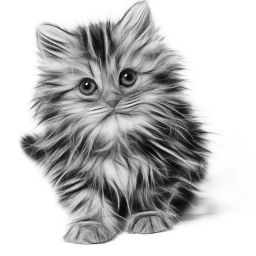
\includegraphics[scale=\myscale,scale=0.4]{images_fiche/chat_gimp_new_photo_0.png}
\end{center}
\begin{center}
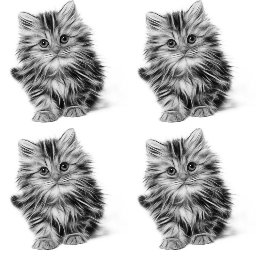
\includegraphics[scale=\myscale,scale=0.3]{images_fiche/chat_gimp_new_photo_1.png}\qquad
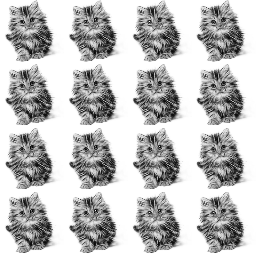
\includegraphics[scale=\myscale,scale=0.3]{images_fiche/chat_gimp_new_photo_2.png}\qquad
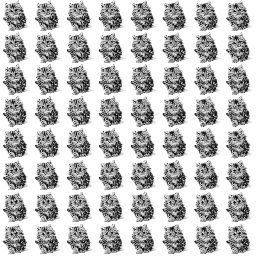
\includegraphics[scale=\myscale,scale=0.3]{images_fiche/chat_gimp_new_photo_3.png}\qquad
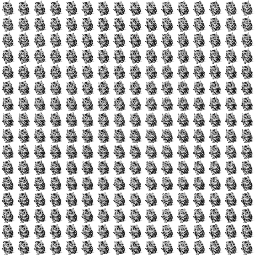
\includegraphics[scale=\myscale,scale=0.3]{images_fiche/chat_gimp_new_photo_4.png}
\end{center}
\begin{center}
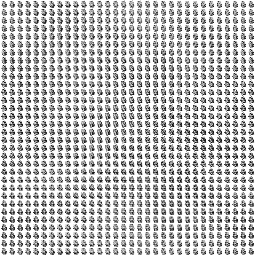
\includegraphics[scale=\myscale,scale=0.3]{images_fiche/chat_gimp_new_photo_5.png}\qquad
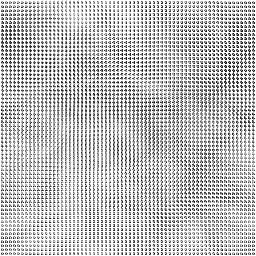
\includegraphics[scale=\myscale,scale=0.3]{images_fiche/chat_gimp_new_photo_6.png}\qquad
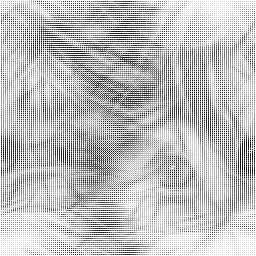
\includegraphics[scale=\myscale,scale=0.3]{images_fiche/chat_gimp_new_photo_7.png}\qquad
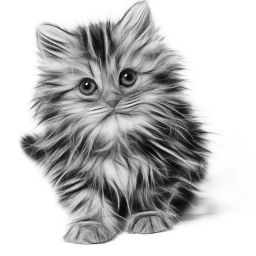
\includegraphics[scale=\myscale,scale=0.3]{images_fiche/chat_gimp_new_photo_8.png}
\end{center}


\end{activite}


%%%%%%%%%%%%%%%%%%%%%%%%%%%%%%%%%%%%%%%%%%%%%%%%%%%%%%%%%%%%%%%%
% Activité 2 - Conversion tableau/image
%%%%%%%%%%%%%%%%%%%%%%%%%%%%%%%%%%%%%%%%%%%%%%%%%%%%%%%%%%%%%%%%


\begin{activite}[Conversion tableau/image]

\objectifs{Objectifs : passer d'un tableau à un fichier d'image et inversement. Le format pour afficher les images est le format \og{}pgm\fg{} qui a été manipulé dans la fiche \og{}Fichiers\fg{}.}

\index{pbm@\emph{pbm/pgm/ppm}}

\begin{enumerate}
  \item \textbf{Tableau vers image.}
  
  Programme une fonction \ci{tableau_vers_image(tableau,nom_image)} qui écrit un fichier image au format \og{}pgm\fg{} à partir d'un tableau de niveaux de gris.
  
\begin{center}
\begin{minipage}{0.3\textwidth}
\begin{lstlisting}
P2
5 5
255
128 192 128 192 128
224   0 228   0 224
228 228 228 228 228 
224  64  64  64 224 
192 192 192 192 192 
\end{lstlisting}
\end{minipage}
\begin{minipage}{0.3\textwidth}
\begin{center}

\includegraphics[scale=\myscale,scale=0.15]{input/ecran-test-pgm}
\end{center}
\end{minipage}
\end{center}
Par exemple avec \ci{tableau = [ [128,192,128,192,128], [224,...] ]}, la commande \ci{tableau_vers_image(tableau,"test")} écrit un fichier \ci{test.pgm} (à gauche) qui s'afficherait comme l'image à droite.

  
  
  \item \textbf{Image vers tableau.} 
  
  Programme une fonction \ci{image_vers_tableau(nom_image)} 
  qui à partir d'un fichier image au format \og{}pgm\fg{}, renvoie un tableau des niveaux de gris.
\end{enumerate}

\end{activite}


%%%%%%%%%%%%%%%%%%%%%%%%%%%%%%%%%%%%%%%%%%%%%%%%%%%%%%%%%%%%%%%%
%%%%%%%%%%%%%%%%%%%%%%%%%%%%%%%%%%%%%%%%%%%%%%%%%%%%%%%%%%%%%%%%
\begin{cours}[Transformation du boulanger]

On part d'un tableau $n\times n$, avec $n$ pair dont chaque élément représente un pixel. 
On va appliquer deux transformations élémentaires à chaque fois :

\begin{itemize}
  \item \textbf{Étirer.} Le principe est le suivant : les deux premières lignes (chacune de longueur $n$) produisent une seule ligne de longueur $2n$ en mixant les valeurs de chaque ligne en alternant un élément du haut, un élément du bas.

\medskip
 
\myfigure{1}{
\tikzinput{fig-images-2}
}

Voici comment deux lignes se mixent en une seule :
\myfigure{1}{
\tikzinput{fig-images-2bis}
}  

\medskip

\emph{Formules.} Un élément en position $(i,j)$ du tableau d'arrivée, correspond à un élément $(2i,j//2)$ (si $j$ est pair) ou bien $(2i+1,j//2)$ (si $j$ est impair) du tableau de départ, avec ici $0 \le i < \frac n2$ et $0 \le j < 2n$.

\medskip

\emph{Exemple.} Voici un tableau $4 \times 4$ à gauche, et le tableau étiré $2 \times 8$ à droite.
Les lignes $0$ et $1$ à gauche donnent la ligne $0$ à droite.
Les lignes $2$ et $3$ à gauche donne la ligne $1$ à droite.
$$\begin{array}{cccc} 
  1& 2& 3& 4\\ 
  5& 6& 7& 8\\  
  9&10&11&12\\  
 13&14&15&16  
\end{array}\qquad\qquad 
\begin{array}{cccccccc} 
  1& 5& 2& 6& 3& 7& 4& 8  \\
  9&13&10&14&11&15&12&16
\end{array}$$
  
  \item \textbf{Replier.} Le principe est le suivant : la partie droite d'un tableau étiré est retournée, puis ajoutée sous la partie gauche. Partant d'un tableau $\frac n2 \times 2n$ on obtient un tableau $n \times n$.

 
\myfigure{0.7}{
\tikzinput{fig-images-3}
}  

\emph{Formules.} 
Pour $0 \le i < \frac n2$ et $0 \le j < n$ les éléments en position $(i,j)$ du tableau sont conservés.
Pour $\frac n2 \le i < n$ et $0 \le j < n$ un élément du tableau 
d'arrivée $(i,j)$, correspond à un élément $\big(\frac{n}{2} - i - 1,2n-1-j\big)$ du tableau de départ. 


\emph{Exemple.} 
À partir du tableau étiré $2 \times 8$ à gauche, on obtient un tableau replié $4 \times 4$ à droite. 
$$ 
\begin{array}{cccccccc} 
  1& 5& 2& 6& 3& 7& 4& 8  \\
  9&13&10&14&11&15&12&16
\end{array}\qquad\qquad
\begin{array}{cccc} 
  1& 5& 2& 6\\ 
  9& 13& 10& 14\\  
  16&12&15&11\\  
  8&4&7&3  
\end{array}$$
\end{itemize}


La \defi{transformation du boulanger} est la succession d'un étirement et d'un repliement. Partant d'un tableau $n \times n$ on obtient encore un tableau $n \times n$.


Voyons un exemple de l'action de plusieurs transformations du boulanger.
À gauche l'image initiale de taille $128 \times 128$, puis le résultat de $k=1,2,3$ itérations. 

\begin{center}
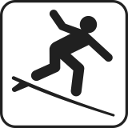
\includegraphics[scale=\myscale,scale=0.65]{images_fiche/surf_gimp_new_boul_0.png}\qquad
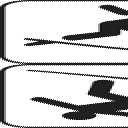
\includegraphics[scale=\myscale,scale=0.65]{images_fiche/surf_gimp_new_boul_1.png}\qquad
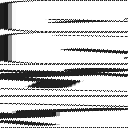
\includegraphics[scale=\myscale,scale=0.65]{images_fiche/surf_gimp_new_boul_2.png}\qquad
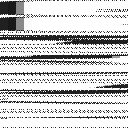
\includegraphics[scale=\myscale,scale=0.65]{images_fiche/surf_gimp_new_boul_3.png}
\end{center}


Voici les images pour $k=12,13,14,15$ itérations :

\begin{center}
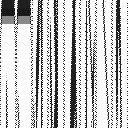
\includegraphics[scale=\myscale,scale=0.65]{images_fiche/surf_gimp_new_boul_12.png}\qquad
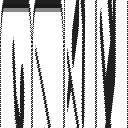
\includegraphics[scale=\myscale,scale=0.65]{images_fiche/surf_gimp_new_boul_13.png}\qquad
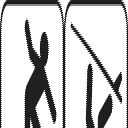
\includegraphics[scale=\myscale,scale=0.65]{images_fiche/surf_gimp_new_boul_14.png}\qquad
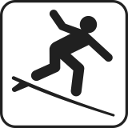
\includegraphics[scale=\myscale,scale=0.65]{images_fiche/surf_gimp_new_boul_15.png}
\end{center}

\end{cours}

%%%%%%%%%%%%%%%%%%%%%%%%%%%%%%%%%%%%%%%%%%%%%%%%%%%%%%%%%%%%%%%%
% Activité 3 - Transfomation du boulanger
%%%%%%%%%%%%%%%%%%%%%%%%%%%%%%%%%%%%%%%%%%%%%%%%%%%%%%%%%%%%%%%%


\begin{activite}[Transformation du boulanger]

\objectifs{Objectifs : programmer une nouvelle transformation qui étire puis replie une image. Encore une fois l'image se déforme de plus en plus mais, au bout d'un certain nombre d'itérations, on retrouve l'image de départ.}


\begin{enumerate}
  \item Programme une fonction \ci{boulanger_etirer(tableau)} qui renvoie un nouveau tableau obtenu en \og{}étirant\fg{} le tableau donné en entrée.



    \item Programme une fonction \ci{boulanger_replier(tableau)} qui renvoie un  tableau obtenu en \og{}repliant\fg{} le tableau donné en entrée.
  
  
   \item Programme une fonction \ci{boulanger_iterer(tableau,k)} qui renvoie le tableau calculé après $k$ itérations de la transformation du boulanger.
  
  Par exemple, voici un tableau $4 \times 4$ à gauche, son image par la transformation ($k=1$) et son image après une seconde transformation ($k=2$).
  
 $$\begin{array}{cccc} 
  1& 2& 3& 4\\ 
  5& 6& 7& 8\\  
  9&10&11&12\\  
 13&14&15&16  
\end{array}\qquad\qquad  
 \begin{array}{cccc} 
  1& 5& 2& 6\\ 
  9& 13& 10& 14\\  
  16&12&15&11\\  
  8&4&7&3  
\end{array}\qquad\qquad  
 \begin{array}{cccc} 
   1&    9&    5&   13 \\ 
 16&    8&   12&    4\\  
  3&   11&    7&   15\\  
 14&    6&   10&    2
\end{array}
$$ 
  \item Programme une fonction \ci{boulanger_images(nom_image,kmax)} qui calcule 
  les images correspondant à la transformation du boulanger, avec des itérations allant de $k=1$ à $k=k_{\max}$.
  
  \item Expérimente pour différentes valeurs de la taille $n$, afin de voir au bout de combien d'itérations on retrouve l'image de départ. 
  
  \emph{Attention !} Il faut parfois itérer beaucoup avant de retrouver l'image de départ. Par exemple avec $n=4$, on retrouve l'image de départ au bout de $k=5$ itérations, avec $n=256$ c'est $k=17$. Conjecture une valeur de retour dans le cas où $n$ est une puissance de $2$. Par contre pour $n=10$, il faut $k = 56\,920$ itérations !
   
  
\end{enumerate}

Voici un exemple avec une image de taille $256 \times 256$, d'abord l'image initiale, puis une première itération ($k=1$) et une deuxième itération ($k=2$).
\begin{center}
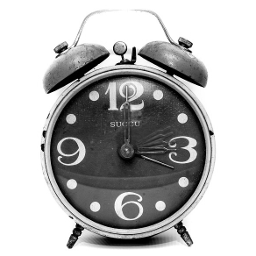
\includegraphics[scale=\myscale,scale=0.4]{images_fiche/reveil_gimp_new_boul_0.png}\qquad
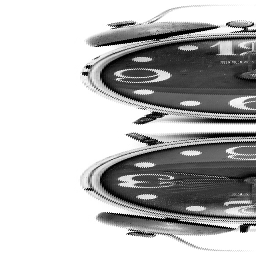
\includegraphics[scale=\myscale,scale=0.4]{images_fiche/reveil_gimp_new_boul_1.png}\qquad
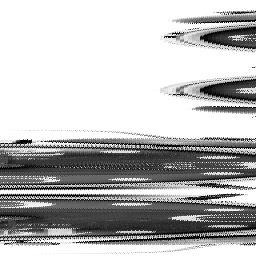
\includegraphics[scale=\myscale,scale=0.4]{images_fiche/reveil_gimp_new_boul_2.png}
\end{center}
$k=3,4,5$ :
\begin{center}
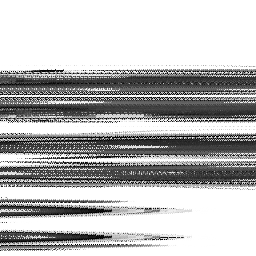
\includegraphics[scale=\myscale,scale=0.4]{images_fiche/reveil_gimp_new_boul_3.png}\qquad
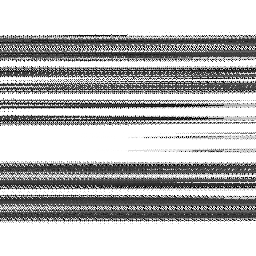
\includegraphics[scale=\myscale,scale=0.4]{images_fiche/reveil_gimp_new_boul_4.png}\qquad
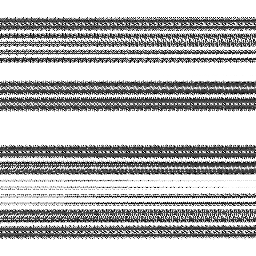
\includegraphics[scale=\myscale,scale=0.4]{images_fiche/reveil_gimp_new_boul_5.png}
\end{center}

$k=15,16,17$ :
\begin{center}
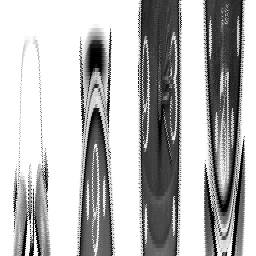
\includegraphics[scale=\myscale,scale=0.4]{images_fiche/reveil_gimp_new_boul_15.png}\qquad
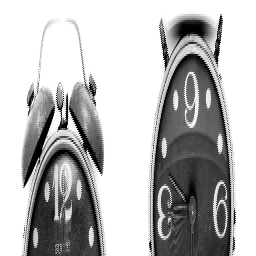
\includegraphics[scale=\myscale,scale=0.4]{images_fiche/reveil_gimp_new_boul_16.png}\qquad
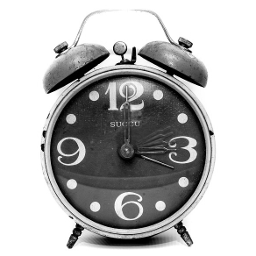
\includegraphics[scale=\myscale,scale=0.4]{images_fiche/reveil_gimp_new_boul_17.png}
\end{center}

Pour $k=17$ on retrouve l'image de départ !

\end{activite}


Cette fiche est basée sur l'article \og{}Images brouillées, images retrouvées\fg{} par Jean-Paul Delahaye et Philippe Mathieu (Pour la Science, 1997).


\end{document}
